\documentclass{article}
\usepackage{amsmath}
\usepackage{listings}
\usepackage{array}
\usepackage{tikz} 
\usepackage{underscore}
\usepackage[bookmarks=true]{hyperref}
\usepackage[utf8]{inputenc}
\usepackage[english]{babel}
\usepackage{enumitem}
\usepackage[a4paper, margin=1in]{geometry}
\usetikzlibrary{shapes, arrows.meta, positioning, backgrounds}

% Define styles for different node types
\tikzstyle{startstop} = [rectangle, rounded corners, minimum width=3cm, minimum height=1cm, text centered, draw=black, fill=red!30]
\tikzstyle{process} = [rectangle, minimum width=3.5cm, minimum height=1cm, text centered, draw=black, fill=blue!30]
\tikzstyle{arrow} = [thick,->,>=stealth]

% Define stickman style
\tikzset{
    stickman/.pic={
        % Head
        \draw[fill=gray] (0,0.6) circle (0.3cm);
        % Body
        \draw[line width=0.5mm] (0,0.3) -- (0,-0.6);
        % Arms
        \draw[line width=0.5mm] (-0.4,0.3) -- (0.4,0.3);
        % Legs
        \draw[line width=0.5mm] (0,-0.6) -- (-0.4,-1.2);
        \draw[line width=0.5mm] (0,-0.6) -- (0.4,-1.2);
    }
}

% Hyperref settings
\hypersetup{
    pdftitle={Software Requirement Specification},
    pdfauthor={Jean-Philippe Eisenbarth},
    pdfsubject={TeX and LaTeX},
    pdfkeywords={TeX, LaTeX, graphics, images},
    colorlinks=true,
    linkcolor=blue,
    citecolor=black,
    filecolor=black,
    urlcolor=purple,
    linktoc=page
}

% Set extra row height and padding
\setlength{\extrarowheight}{4pt}
\renewcommand{\arraystretch}{1.5}

\begin{document}

\begin{titlepage}
    \centering
    \includegraphics[width=0.5\textwidth]{logo.png} % Adjust width as necessary
    \vspace{1cm}

    \textbf{Department of Computer Science and Engineering}\\
    Premier University
    \vspace{1cm}

    \huge \textnormal{MGT 251: Organizational Behavior }
    \vspace{1in} 

    \Large \textnormal{Title: CT-02 Assignment}
    \vspace{0.5in} % Adjusts vertical space after the assignment title

    \large
    \textbf{Submitted by:}
    \vspace{0.5cm}

    \renewcommand{\arraystretch}{1.5} % Adjusts vertical spacing in the table
    \begin{tabular}{|p{0.4\textwidth}|p{0.6\textwidth}|} % Set column widths to 40% and 60%
        \hline
        \textbf{Name} & Mohammad Hafizur Rahman Sakib \\
        \hline
        \textbf{ID} & 0222210005101118 \\
        \hline
        \textbf{Section} & C \\
        \hline
        \textbf{Session} & Spring 2024 \\
        \hline
        \textbf{Semester} & 5th Semester \\
        \hline
        \textbf{Submission Date} & 17.09.2024 \\
        \hline
    \end{tabular}
    \vspace{1cm}

    \begin{minipage}[t]{0.48\textwidth}
        \textbf{Submitted to:}\\
        Jafrin Sabrina\\
        Lecturer, Business Administration\\
        Premier University\\
        Chittagong
    \end{minipage}%
    \hfill
    \begin{minipage}[t]{0.48\textwidth}
        \raggedleft
        \textbf{Remarks}\\
        \vspace{0.5cm} % Adjust vertical space for remarks
        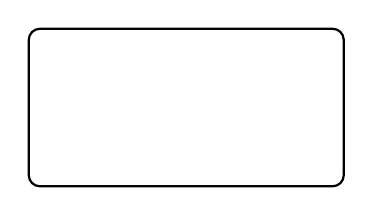
\begin{tikzpicture}
            \draw[thick, rounded corners] (0,0) rectangle (4,2);
        \end{tikzpicture}
    \end{minipage}

    \date{\today}
    \vfill
\end{titlepage}
\section*{Q.1 How does Attribution theory influence a person’s judgment decision? Describe this with a real-life scenario.}

Attribution theory is a psychological framework that examines how individuals interpret the causes of behavior and events. In organizational behavior, it plays a critical role in shaping the judgments and decisions made by managers and employees alike. This theory was developed by Fritz Heider, who proposed that individuals tend to seek reasons for other people's actions by attributing them to either internal or external causes.

\subsection*{Types of Attribution}
Attribution can be categorized into two types: internal attribution and external attribution.

\begin{itemize}
    \item \textbf{Internal Attribution:} When people attribute behavior to personal factors such as traits, abilities, or effort, they are engaging in internal attribution. For example, if an employee completes a project ahead of schedule, their manager might attribute this success to the employee's strong work ethic or intelligence.
    \item \textbf{External Attribution:} On the other hand, when behavior is attributed to situational or environmental factors, it is known as external attribution. For instance, if the same employee misses a deadline, the manager might attribute the failure to external factors such as technical difficulties or unrealistic expectations.
\end{itemize}

\subsection*{The Role of Attribution in Judgment and Decision-Making}
In organizational settings, attribution theory has a profound impact on how managers evaluate the performance and behavior of their employees. The judgments made based on attribution can lead to important decisions, such as promotions, performance appraisals, and even disciplinary actions.

\textbf{Internal Attribution in the Workplace:}  
Managers often make internal attributions when evaluating employee performance. For example, if an employee consistently produces high-quality work, the manager may attribute this success to the employee's personal qualities such as diligence, creativity, or expertise. This positive attribution can lead to rewards like promotions, bonuses, or leadership opportunities.

However, internal attribution can also work against employees. If a manager perceives an employee's failure as a reflection of their lack of effort or incompetence, they may be less inclined to provide support or understanding. This can create a negative cycle where the employee's future performance is scrutinized more harshly, and their career development is hindered.

\textbf{External Attribution in the Workplace:}  
External attributions, on the other hand, allow managers to take a more compassionate and nuanced approach to employee performance. For example, if an employee fails to meet a deadline, a manager who considers external factors, such as a heavy workload or family emergencies, may be more likely to offer assistance or extend deadlines. This understanding approach fosters a supportive work environment where employees feel valued and respected.

\subsection*{Attribution Bias}
Attribution bias occurs when individuals consistently favor one type of attribution over another, often leading to distorted judgments. Some common types of attribution bias include:

\begin{itemize}
    \item \textbf{Fundamental Attribution Error:} This bias occurs when people overemphasize internal factors and underestimate external factors when evaluating others' behavior. For example, a manager might blame an employee's lateness on laziness (internal attribution) without considering traffic problems (external attribution).
    \item \textbf{Self-Serving Bias:} This occurs when individuals attribute their own successes to internal factors and their failures to external factors. For example, an employee might attribute a successful project to their own abilities, but blame failure on lack of resources.
    \item \textbf{Actor-Observer Bias:} This bias happens when individuals attribute their own actions to external factors but attribute others' actions to internal factors. A manager might excuse their own shortcomings by pointing to external pressures but blame an employee’s underperformance on their personality or work ethic.
\end{itemize}

\subsection*{Real-life Scenario:}
Consider the case of a sales team where one member, John, consistently underperforms compared to his peers. John's manager, Sarah, must decide how to address his performance issues. According to attribution theory, Sarah could make either an internal or external attribution.

\textbf{Internal Attribution Example:}  
If Sarah attributes John's poor performance to internal factors, she might assume that he lacks motivation or skills. As a result, Sarah might decide to place John on a performance improvement plan or even consider termination if his performance does not improve. This judgment could lead to strained relationships within the team, as John may feel unfairly treated if his struggles are due to factors beyond his control.

\textbf{External Attribution Example:}  
Alternatively, Sarah might consider external factors, such as John's recent health issues or increased family responsibilities. In this case, she might offer him more flexibility, additional training, or workload adjustments. This external attribution fosters a more supportive work environment, encouraging John to improve his performance without feeling blamed or judged.

In both cases, the attribution Sarah makes will significantly influence her judgment and the decisions she makes regarding John's future in the company. Incorrect attributions can lead to unfair decisions, while balanced attributions can promote fairness and growth within the organization.

\subsection*{Impact of Attribution Theory on Decision-Making}
Attribution theory has profound implications for decision-making in organizations. Managers must be aware of their own attribution tendencies to avoid biased judgments that could harm employee morale and productivity. For example, a manager who consistently makes internal attributions might develop a reputation for being overly critical, causing employees to feel undervalued or stressed. Conversely, a manager who frequently makes external attributions might be seen as too lenient, which could affect team performance.

In conclusion, attribution theory highlights the importance of understanding the root causes of behavior in organizational settings. Managers and employees alike must be mindful of their attribution biases to foster a fair and supportive work environment.

% \newpage

\section*{Q.2 Analyze the influence of Halo Effect and Contrast Effect on organizational behavior}

The Halo Effect and Contrast Effect are two common cognitive biases that significantly impact perceptions and decision-making within organizations. These biases can influence how employees are evaluated, how teams function, and how leadership decisions are made.

\subsection*{Halo Effect}
The Halo Effect refers to the tendency to let one positive attribute of an individual influence the overall perception of their abilities and traits. This bias can lead to overgeneralization, where one outstanding quality overshadows other aspects of the individual’s performance.

\subsection*{Impact of Halo Effect on Organizational Behavior}
The Halo Effect is pervasive in organizations, particularly in performance appraisals, recruitment, and promotions. For instance, if a manager is impressed by an employee’s punctuality, they might assume that the employee is also highly efficient, diligent, and competent in other areas of work. This could lead to the employee receiving higher performance ratings across the board, even if their actual work quality is average in some areas.

\textbf{Example:}  
Consider an employee, Jane, who consistently arrives on time and maintains a professional demeanor in meetings. Due to this, her manager develops a highly favorable impression of her, assuming that she is equally proficient in all areas of her job. Even if Jane’s actual work performance in technical skills or project management is not as strong, she might still be rated highly in those areas due to the Halo Effect.

\textbf{Consequences of the Halo Effect:}  
The Halo Effect can lead to various organizational consequences:

\begin{itemize}
    \item \textbf{Biased Performance Evaluations:} Employees who excel in one visible area may be rated highly across all categories, while others who perform well but lack a standout trait might be overlooked.
    \item \textbf{Unfair Promotions:} Employees may be promoted based on one strong characteristic rather than an overall assessment of their skills, leading to mismatched job roles and underperformance.
    \item \textbf{Team Dynamics:} The Halo Effect can affect team dynamics, as some members might receive undue recognition, creating resentment among colleagues.
\end{itemize}

\subsection*{Contrast Effect}
The Contrast Effect occurs when an individual’s performance is judged in comparison to others, rather than being evaluated on their own merits. This bias can significantly affect how employees are perceived, especially in competitive environments like performance reviews or recruitment.

\subsection*{Impact of Contrast Effect on Organizational Behavior}
The Contrast Effect can distort evaluations by exaggerating the differences between employees. For example, if an average performer is evaluated immediately after a top performer, they may appear less competent than they actually are. This bias can lead to inaccurate assessments and unfair treatment of employees.

\textbf{Example:}  
Imagine two employees, Mark and Sarah, being interviewed for a promotion. Mark is interviewed first and gives an outstanding performance, showcasing his extensive knowledge and experience. When Sarah is interviewed next, even though she is highly competent, her performance may seem less impressive in comparison to Mark’s. As a result, the interviewer may rate her lower than she deserves, purely due to the comparison with Mark.

\textbf{Consequences of the Contrast Effect:}  
The Contrast Effect can have several negative consequences in organizational settings:

\begin{itemize}
    \item \textbf{Inaccurate Hiring Decisions:} Candidates may be unfairly judged based on how they compare to others in the interview process, rather than being assessed on their own qualifications and fit for the role.
    \item \textbf{Distorted Performance Reviews:} Employees who follow high performers may receive lower ratings than they deserve, while those who follow weaker performers may receive higher ratings.
    \item \textbf{Reduced Employee Morale:} Employees who feel unfairly compared to their peers may become demotivated, leading to reduced productivity and engagement.
\end{itemize}

\subsection*{Managing Halo and Contrast Effects in Organizations}
Organizations can mitigate the influence of the Halo Effect and Contrast Effect by implementing objective, structured evaluation processes. Some strategies include:

\begin{itemize}
    \item \textbf{Use of Objective Criteria:} Basing evaluations on specific, measurable criteria rather than subjective impressions can help reduce the influence of cognitive biases.
    \item \textbf{Training for Managers:} Providing training to managers on common cognitive biases can increase awareness and help them make more balanced judgments.
    \item \textbf{Peer Reviews and 360-Degree Feedback:} Incorporating multiple perspectives in performance evaluations can provide a more holistic and accurate view of an employee’s abilities.
    \item \textbf{Continuous Evaluation:} Conducting regular performance assessments rather than one-time reviews can prevent the recency bias associated with the Contrast Effect.
\end{itemize}

\end{document}